\documentclass[amssymb,twocolumn,aps]{revtex4}

% allows special characters (including æøå)
\usepackage[utf8]{inputenc}
%\usepackage [norsk]{babel} %if you write norwegian
\usepackage[english]{babel}  %if you write english

\usepackage{physics,amssymb}  % mathematical symbols (physics imports amsmath)
\usepackage{graphicx}         % include graphics such as plots
\usepackage[table]{xcolor}
\usepackage{xcolor}           % set colors
\usepackage{hyperref}         % automagic cross-referencing 
\usepackage{float}			  % force placement of tables and figures

\begin{document}
	
\title{Report Template \\
    \normalsize FYS-STK3155 - Project X}
\date{\today}               
\author{Student}
\affiliation{University of Oslo}

\newpage
	
\begin{abstract}
In this project, we investigate the application of supervised machine learning techniques to regression problems, with a particular focus on understanding the bias--variance trade-off and the effects of regularization. Using synthetic and real-world datasets, we implement and compare Ordinary Least Squares (OLS) and Ridge regression models across varying levels of model complexity and regularization strength. Our results demonstrate how model selection and hyperparameter tuning influence prediction accuracy, and we visualize these effects through informative figures. The findings provide practical insights into balancing bias and variance for optimal model performance.
\end{abstract}

\maketitle

\section{Introduction}
Machine learning has become an essential tool for analyzing and modeling complex data across science and industry. In regression analysis, the goal is to predict a continuous outcome variable from one or more input features, while avoiding both underfitting and overfitting. Achieving robust generalization requires careful control of model complexity and a clear understanding of the bias--variance trade-off. In this project, we explore these concepts by implementing and evaluating Ordinary Least Squares (OLS) and Ridge regression. We systematically study how polynomial model degree and regularization strength (ridge penalty) affect prediction error measured by mean squared error (MSE). To make these effects tangible, we present visualizations of the bias--variance trade-off and a heatmap of MSE across degrees and regularization parameters. Together, these results illustrate how model selection and hyperparameter tuning can improve predictive performance.

The rest of the report is organized as follows. Section~\ref{section:methods} describes the methods and implementation details used in our experiments. Section~\ref{section:results} presents and discusses the results, including the figures that illustrate the trade-offs inherent to model complexity and regularization. Finally, Section~\ref{section:conclusion} summarizes the main findings and outlines potential directions for future work.
    
\section{Methods}\label{section:methods}

\subsection{Method 1/X}

\begin{itemize}
    \item Describe the methods and algorithms, including the motivation for using them and their applicability to the problem
    \item Derive central equations when appropriate, the text is the most important part, not the equations.
\end{itemize}

\subsection{Implementation}

\begin{itemize}
    \item Explain how you implemented the methods and also say something about the structure of your algorithm and present very central parts of your code, not more than 10 lines
    \item You should plug in some calculations to demonstrate your code, such as selected runs used to validate and verify your results. A reader needs to understand that your code reproduces selected benchmarks and reproduces previous results, either numerical and/or well-known closed form expressions.
\end{itemize}

\subsection{Use of AI tools}

We used ChatGPT to assist with drafting text and troubleshooting minor coding issues. All generated suggestions were reviewed, verified, and edited by us to ensure correctness and relevance to the project.
	
\section{Results and Discussion}\label{section:results} 

\begin{itemize}
    \item Present your results
    \item Give a critical discussion of your work and place it in the correct context.
    \item Relate your work to other calculations/studies
    \item An eventual reader should be able to reproduce your calculations if she/he wants to do so. All input variables should be properly explained.
    \item Make sure that figures and tables contain enough information in their captions, axis labels etc. so that an eventual reader can gain a good impression of your work by studying figures and tables only.
    \item Figure \ref{fig:bvt} illustrates the bias-variance tradeoff, demonstrating how model complexity affects the balance between bias and variance in predictive modeling.
    \item Figure \ref{fig:mse_heatmap} shows the MSE of a Ridge regression model for various polynomial degrees and lambda values, highlighting how regularization strength impacts model performance across different complexity levels.
\end{itemize}

\begin{figure}[h]
    \centering
    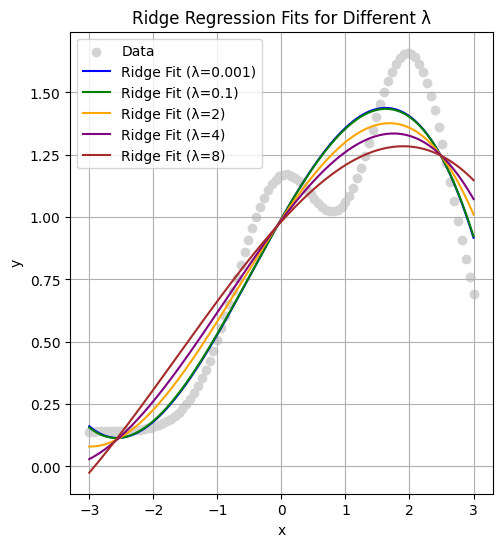
\includegraphics[width=0.5\linewidth]{Figures/bvt.png}
    \caption{Variance tradeoff for different normalizing values of lambda.}
    \label{fig:bvt}
\end{figure}
\begin{figure}[h]
    \centering
    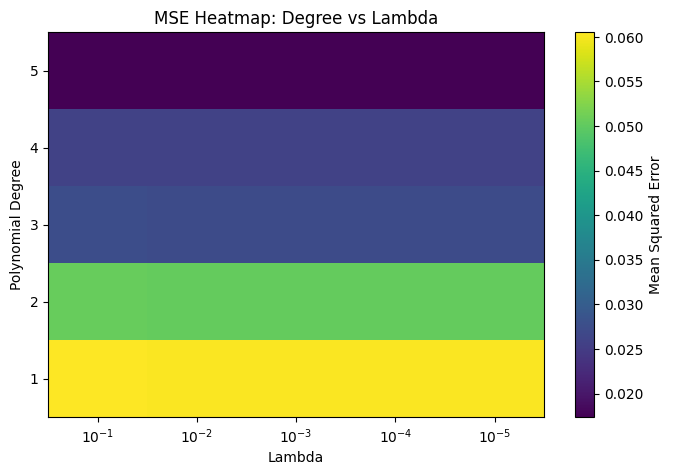
\includegraphics[width=1.0\linewidth]{Figures/mse_heatmap.png}
    \caption{Heatmap showing the MSE of a Ridge regression model for various polynomial degrees and lambda values.}
    \label{fig:mse_heatmap}
\end{figure}

\section{Conclusion}\label{section:conclusion} 
\begin{itemize}
    \item State your main findings and interpretations
    \item Try to discuss the pros and cons of the methods and possible improvements
    \item State limitations of the study
    \item Try as far as possible to present perspectives for future work
\end{itemize}

\bibliography{biblio}

\end{document}
